\chapter{The \emph{Expedition} software suite: Computational tools for transcriptome analysis}


% From main text: We developed Expedition, a suite of algorithms integrated in a complete software package designed to address three key concepts that are critical for single-cell analyses: (1) rejection of an alternative event if its definition is incompatible with the data, and (2) ability to describe the variation of AS such as detect bimodality and (3) visualize AS distribution changes from one cell type or state to another.

In this paper, we developed the \emph{Expedition} suite, consisting of  software packages that addressed three key deficiencies in single-cell alternative splicing analysis:

\begin{enumerate}
	\item \textbf{Detect and quantify alternative splicing quickly, with minimum false positives: \outrigger, \Cref{sec:outrigger}}\\
	In single-cell analysis, absolute quantitation of gene expression or ``percent spliced-in'' (Psi/$\Psi$) is important and enable us to learn the distribution of these quantitations. Previously, relative quantitation for splicing ($\Delta\Psi$) is more commonly used to calculate the difference between groups. Such relative quantitation tolerates false positive better, as false positives may not vary between groups, $\Delta\Psi \sim 0$ and are thus not noticeable in pairwise comparisons. However, when studying distribution of absolute quantitation, such false positives obscure the observation in unpredictable way and hinder biological interpretation. The second main problem of previous splicing algorithm is the inflexible definitions of alternative exons. The same alternative exons may utilize different flanking exons in different cells/samples, thus leading to different biological interpretation. To address these problems, we create \outrigger, which uses junction reads to find de novo exons, creates a splice graph to define junction-based alternative events, filters for conserved splice sites, and strictly rejectes cases of alternative events incompatible with the data at hand. Finally, we discuss and compare to the popular MISO\cite{Katz:2010iv} algorithm.
	\item \textbf{Classify modalities of alternative splicing events, including bimodal: \anchor, \Cref{sec:anchor}}\\
	The power of single-cell analyses rises from the ability to study the distribution of a parameter-of-interest. There are a few statistical methods for finding bimodal distributions, but none are sufficient because they are either not sensitive enough, or not robust enough to noise. Additionally, these methods only deal with bimodal distribution and do not classify other distributions, such as unimodal or multimodal. To create a sensitive distribution classifier for all modalities, we used Bayesian methods to create \anchor, and compare our method to a simple binning method, the bimodality index\cite{Wang:2009wm}, and the bimodal dip test\cite{Hartigan:1985ca}.
	\item \textbf{Quantify and visualize dynamics in distributions: \bonvoyage,\linebreak \Cref{sec:bonvoyage}}\\
	While there are many statistical tests to compare changes in distributions, few of them is coupled with visual tools to present changes in distribution with both magnitude and direction. For the specific question of alternative splicing changes, we are interested in observing a event becomes more included or more excluded. Thus we have employed machine learning methods to create a visualizable, interpretable 2d space with ``included'' and ``excluded'' axes. This method is compared to the quantification offered by the Jensen-Shannon Divergence (JSD)\cite{Cover:2011vn}.
\end{enumerate}

\section{\texttt{outrigger}: Splicing estimation with \emph{de novo} annotation and graph traversal}
\label{sec:outrigger}

Currently available tools for AS detection and quanitification have two major problems: (1) inflexible definitions that cannot handle different configurations of flanking exons for the same alternative junctions, and (2) lack of rejection of an alternative event even if its definition is incompatible with the data-at-hand. The first problem is solved with \texttt{outrigger index}, which defines all potential alternative events based on the junctions and alternative exons from the aggregate of entire sample sets in a given project, and enumerates all biologically possible flanking exon combinations. This step maximize the likelihood to identify all possible alternative events. To ensure only valid alternative events were generated, we added \texttt{outrigger validate} to remove alternative events with introns lacking conserved splice sites. The second prolbem is solved with \texttt{outrigger psi}, which applies strict rules to only permit junctions with sufficient coverage for an event in a given sample. All the parameters in the rules can be user-defined. Thus, outrigger addresses key issues with current alternative splicing software.

\subsection{Algorithm overview}

Broadly, the goal of \outrigger\, is to create a custom, \emph{de novo} alternative splicing annotation by using junction reads and exon definitions to create a exon-junction graph, traversing the graph to find alternative events, and calculate percent spliced-in (Psi/$\Psi$) of the alternative exons.


\begin{figure}[h]
  \centering
  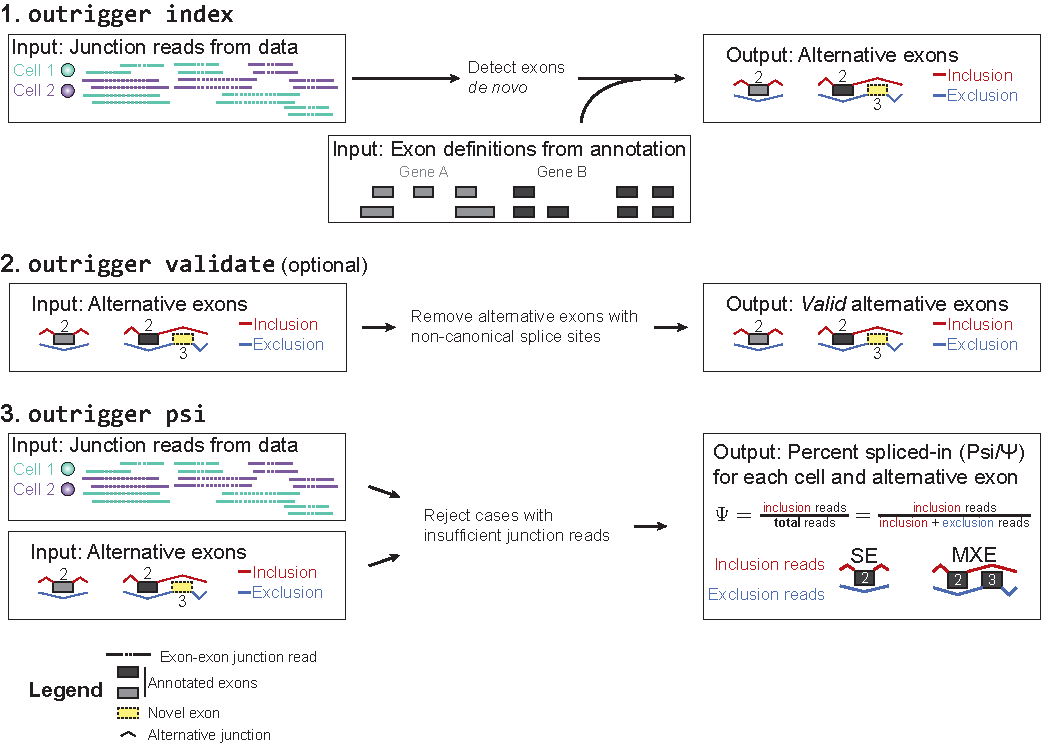
\includegraphics[width=5.6in]{figures/outrigger_overview.pdf}
  \caption[Overview of \outrigger's three steps and associated commands: indexing (\texttt{outrigger index}), validation (\texttt{outrigger validate}) and percent spliced-in (Psi/$\Psi$) calculation (\texttt{outrigger psi})]{Overview of \outrigger's three steps and associated commands: indexing (\texttt{outrigger index}), validation (\texttt{outrigger validate}) and percent spliced-in (Psi/$\Psi$) calculation (\texttt{outrigger psi}). In the first step of building an index, \outrigger\, considers the entirety of junction reads from the user-input dataset to detect exons \emph{de novo}, adds annotated exons, then searches for alternative exons. In the second, optional, step of validating the detected events, \outrigger\, removes alternative exons with flanking introns lacking consensus splice sites. For the third step of calculating Psi/$\Psi$, \outrigger\, utilizes junction reads together with alternative exons defined in the indexing step and calculates $\Psi$ for each sufficiently covered event. Only junction reads are used to represent inclusion or exclusion reads. SE, Skipped Exon; MXE, Mutually Exclusive Exons.
  }
  \label{fig:outrigger_overview}
\end{figure}




\paragraph{\texttt{outrigger index}: Create custom alternative splicing annotation.} The following is a narrative describing \textbf{\Cref{fig:outrigger_index}a}.


% --- BEGIN manual facingcaption --- %
\clearpage
\thispagestyle{facingcaption}
\begin{figure}[h]
\captionsetup{labelformat=prev-page}
  \caption[Internal steps of indexing via \texttt{outrigger index}: Exons identification and defining alternative events.]{
  Internal steps of indexing via \texttt{outrigger index}: Exons identification and defining alternative events.\\
% \captionof{figure}{\textbf{} \\
\textbf{a.} Internal workings of the indexing step via \texttt{outrigger index}. User-provided inputs junction reads can be either genome-aligned \texttt{.bam} files, the \texttt{.SJ.out.tab} splice junction files from the STAR aligner, or a compiled table in \texttt{.csv} of all junction reads from all samples for the project. Step 1, only junction reads with sufficient depth in a cell/sample are retained. By default, the minimum number of reads is $10$ per cell/sample, which can be modified with the flag \texttt{-{}-min-reads}. Step 2, junction reads are used to identify junction locations, and reads are aggregated across all cells/samples regardless of which cell/sample it came from. Step 3, if there is a ``gap'' between two junctions that is smaller than certain length $X$ (by default, $X=100$ nucleotides but can be modified with the flag \texttt{-{}-max-de-novo-exon-length}), then an exon is inserted. Step 4, the identified exons are compared with the annotated exons to obtain the pairwise relationships between exons and junctions. Step 4 outputs a table of ``triples:'' of \texttt{(exon, direction, junction)} encoding the directional relationship between exons and junctions. Step 5, the output tables from step 4 are utilized to connect exons through junctions and creates a graph database. Finally, in Step 6, alternative exons are identified by traversing the graph database. The output of the indexing step run by the command \texttt{outrigger index}, is junction-based, outputting the alternative exon and all possible configurations of flanking exons for each event. For example, on the bottom right, the same skipped exon event using the same alternative junctions, have four possible configurations of flanking exons. They are considered to be the same event, but are reported with all four configurations for the ease-to-use in downstream analysis.\\
\textbf{b.} Defining alternative events and comparison of biological interpretability of events found by MISO and \outrigger. For a given alternative exon (black box), there can be multiple transcripts corresponding to the alternative exon but with different flanking exons. MISO chooses to define the alternative event using the shortest exons on both sides. Yet, this MISO-defined alternative event may not actually exist as a transcript in the dataset and will be misleading to interpret. For example, attempts to translate such non-existing transcript(s) will be inappropriate. In contrast, \outrigger\, defines the event based on the junctions, and outputs all corresponding flanking exon configurations, thus enabling broader use of the outputs and more relevant biological interpretation.
}
\label{fig:outrigger_index}
\end{figure}
\clearpage
\begin{figure}[h]
\ContinuedFloat
\captionsetup{labelformat=empty}
\centering
% \includegraphics[width=5.8in]{sandiego.jpg}
  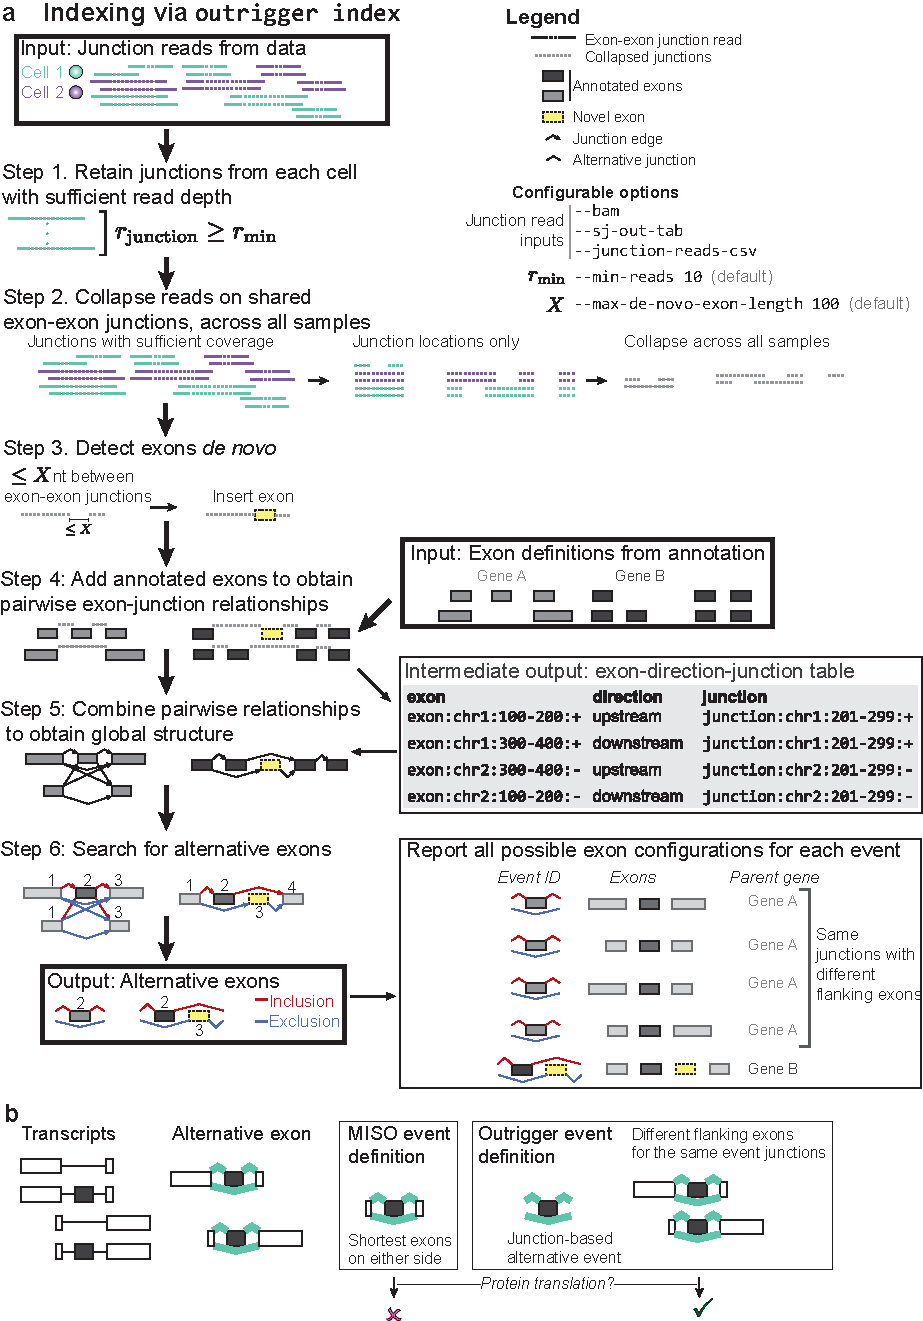
\includegraphics[width=5.8in]{figures/outrigger_index}
\end{figure}
%and, I'm not sure why, but one of the times I used this code the figure number wasn't augmented for the next figure, so check your figure numbers and if necessary uncomment the following line
\addtocounter{figure}{1}
\clearpage
% --- END manual facingcaption --- %


\subparagraph{Inputs.} Two inputs are required for \texttt{outrigger index}: junction counts and gene annotations. The junction counts can be provided in many forms: either \texttt{.bam} \cite{Group:OEYDIUUE} genome alignment files, splice junction count \texttt{.SJ.out.tab} files created by the STAR aligner\cite{Dobin:2013fg}, or a pre-compiled table of samples' junction reads in a \texttt{.csv} format. The gene annotations can be provided in \texttt{.gtf} or \texttt{.gff} format.

\subparagraph{Step 1: Retain junctions from each cell with sufficient read depth.} Junctions with reads in an individual sample less than the minimum number of reads, $r_{\min}$ are removed. By default, $r_{\min} = 10$, and can be adjusted by the user, for example to a minimum of 88 reads, with \texttt{-{}-min-reads~88} on the command line. To illustrate, if one junction is observed with two (2) reads in 100 samples, although there were a total of 200 reads observed on the junction, it will be discarded at this step. Because, there is not sufficient evidence to suggest that this junction is well-covered in any sample.

\subparagraph{Step 2: Collapse reads on shared exon-exon junctions, across all samples.} The aggregate of all junctions from all samples in a given project are create to maximize the likelihood of identifing all potential alternative events.

\subparagraph{Step 3: Detect exons \emph{de novo}.} If the gap between two junctions is under $X$ nucleotides, an exon will be inserted at the gap. This maximum $X$ is necessary, because otherwise we could insert ``exons'' that are many kilobases long, but aren't true exons -{}- they are the intergeneic space between genes. By default, $X = 100$, and this can be adjusted by the user, for example to 157 nucleotides, with the command line flag, \texttt{-{}-max-de-novo-exon-length~157}.

\subparagraph{Step 4: Integrate exon annotation to obtain pairwise exon-junction relationships.} Annotated exons are integrated with the \emph{de novo} exons and create a table of the pairwise relationships of each exon to each junction. We do this by creating a database of genes, transcripts, and exons from a GTF gene annotation file using \texttt{gffutils} \cite{gffutils:sP8uhXuv}, and observing which junctions are adjacent to each exon. This outputs an \emph{``exon-direction-junction''} table which is used in Step 5.

\subparagraph{Step 5: Combine pairwise relationships to obtain global structure.} We then use the adjacencies to build a directional graph which connects exons to each other via junctions. This graph database was built using \texttt{graphlite} \cite{graphlite:vt}, a Python program that provides a lightweight graph wrapper over SQLite.

\subparagraph{Step 6: Search for alternative exons.} To find alternative events, all exons in the graph database were transversed to test, if starting from that exon, it could be a first exon of an skipped exon (SE) or mutually exclusive exon (MXE) event.

\subparagraph{Outputs.} The output of \texttt{outrigger index} is a folder containing the following. The \texttt{events.csv} file contains the event definitions will be used by \texttt{outrigger psi}. The \texttt{exonN.bed} files, where \texttt{N} is an exon number, will be used by \texttt{outrigger validate} to check for canonical or non-canonical splice sites.

The splicing event definitions in the \texttt{events.csv} files are specified by the junctions and the alternative exon. As there may be multiple potential flanking exons with the same junctions, rather than choosing a single version (as is done by MISO, \textbf{\Cref{fig:outrigger_index}b}), we output all possible flanking exon configurations. Thus, while the critical alternative exons are exon 2 for SE events and exons 2 and 3 for MXE events, we show all possible exon flanking exon 1s and exon 3s for SE, and all possible flanking exon 1s and exon 4s for MXE events (\textbf{\Cref{fig:outrigger_index}a}, lower right).

Below is an example command using \texttt{outrigger index}:

\begin{verbatim}
outrigger index -{}-bam *sorted.bam \
    -{}-gtf gencode.vM10.annotation.gtf
\end{verbatim}

This creates a folder called \texttt{outrigger\_output} with the following contents:


\begin{figure}
\footnotesize
\dirtree{%
.1 outrigger\_output/.
.2 index.
.3 gtf\DTcomment{Added by Step 3}.
.4 gencode.vM10.annotation.gtf\DTcomment{Added by Step 4}.
.4 gencode.vM10.annotation.gtf.db\DTcomment{Added by Step 4}.
.4 novel\_exons.gtf\DTcomment{Added by Step 3}.
.3 exon\_direction\_junction.csv\DTcomment{Added by Step 4}.
.3 mxe\DTcomment{Added by Step 6}.
.4 event.bed\DTcomment{Added by Step 6}.
.4 events.csv\DTcomment{Added by Step 6}.
.4 exon1.bed\DTcomment{Added by Step 6}.
.4 exon2.bed\DTcomment{Added by Step 6}.
.4 exon3.bed\DTcomment{Added by Step 6}.
.4 exon4.bed\DTcomment{Added by Step 6}.
.4 intron.bed\DTcomment{Added by Step 6}.
.3 se\DTcomment{Added by Step 6}.
.4 event.bed\DTcomment{Added by Step 6}.
.4 events.csv\DTcomment{Added by Step 6}.
.4 exon1.bed\DTcomment{Added by Step 6}.
.4 exon2.bed\DTcomment{Added by Step 6}.
.4 exon3.bed\DTcomment{Added by Step 6}.
.4 intron.bed\DTcomment{Added by Step 6}.
.2 junctions\DTcomment{Added by Step 1}.
.3 metadata.csv\DTcomment{Added by Step 2}.
.3 reads.csv\DTcomment{Added by Step 1}.
}
\caption{Example output of \texttt{outrigger index} command.}
\end{figure}


Besides outputting the relevant \texttt{events.csv} which is used in \texttt{outrigger psi} to define events, we also output \texttt{.bed} files for the entire event, the alternative intron, and each exon, facilitating downstream sequence analysis.


\paragraph{\texttt{outrigger validate}: Remove alterantive splicing lacking conserved splice sites.} The following describes the biological intuition behind \textbf{\Cref{fig:outrigger_validate_frankenevents}a}. Major (U2) splicesome recognize splice-sites as  ($5^\prime$ end of intron/$3^\prime$ end of intron) \texttt{GT/AG} and \texttt{GC/AG} the Minor (U12) spliceosome recognizes splice-sites as \texttt{AT/AC}\cite{McManus:2011en,GarciaBlanco:2004kl}. By default, these combinations of splice-sties are allowed. But the valid splice sites can be user-specified and changed for example to \texttt{AA/AA} and \texttt{GG/GG} with \texttt{-{}-valid-splice-sites~AA/AA,GG/GG}.

The output of \texttt{outrigger validate} is a \texttt{splice\_sites.csv} folder containing the splice sites, and an additional folder in the splice type folder, called \texttt{validated}, containing filtered \texttt{events.csv} which only contain alternative events with valid splice sites. For example, as a follow up on our previous \texttt{outrigger index} command, we validate the alternative exons with the command,

\begin{verbatim}
outrigger validate -{}-genome mm10 \
    -{}-fasta GRCm38.primary_assembly.genome.fa
\end{verbatim}

This creates the following additions to the \texttt{outrigger\_output} folder:

\begin{figure}
\footnotesize
\dirtree{%
.1 outrigger\_output/.
.2 index.
.3 gtf.
.4 gencode.vM10.annotation.gtf.
.4 gencode.vM10.annotation.gtf.db.
.4 novel\_exons.gtf.
.3 exon\_direction\_junction.csv.
.3 mxe.
.4 event.bed.
.4 events.csv.
.4 exon1.bed.
.4 exon2.bed.
.4 exon3.bed.
.4 exon4.bed.
.4 intron.bed.
.4 splice\_sites.csv\DTcomment{Added by \texttt{outrigger validate}}.
.4 validated\DTcomment{Added by \texttt{outrigger validate}}.
.5 events.csv\DTcomment{Added by \texttt{outrigger validate}}.
.3 se.
.4 event.bed.
.4 events.csv.
.4 exon1.bed.
.4 exon2.bed.
.4 exon3.bed.
.4 intron.bed.
.4 splice\_sites.csv\DTcomment{Added by \texttt{outrigger validate}}.
.4 validated\DTcomment{Added by \texttt{outrigger validate}}.
.5 events.csv\DTcomment{Added by \texttt{outrigger validate}}.
.2 junctions.
.3 metadata.csv.
.3 reads.csv.
}
\caption{Example output of \texttt{outrigger validate} command.}
\end{figure}


\paragraph{Potential ``Franken-events'' created by combining junctions over multiple datasets.} As many junctions may occur spuriously in a single cell (sample), aggregating all junctions across all cells (sample) may create events that were not observed in any individual cell (\Cref{fig:outrigger_validate_frankenevents}b). We wanted to ensure we strictly defined when events were valid or not in these cases.

In the case of SE events, the exon will have $\Psi = \text{NA}$ for the cell with the observed inclusion junctions, since they don't have sufficient reads on both sides of the exon. For the cell with the exclusion junction, it will have $\Psi = 0$ since no inclusion reads were observed.

For MXE events, if each of the four junctions was observed independently in a different cell, then all of the cells will have $\Psi = \text{NA}$ for that splicing event since there are no cells which have sufficient reads on all junctions of either isoform.

\begin{figure}
  \centering
  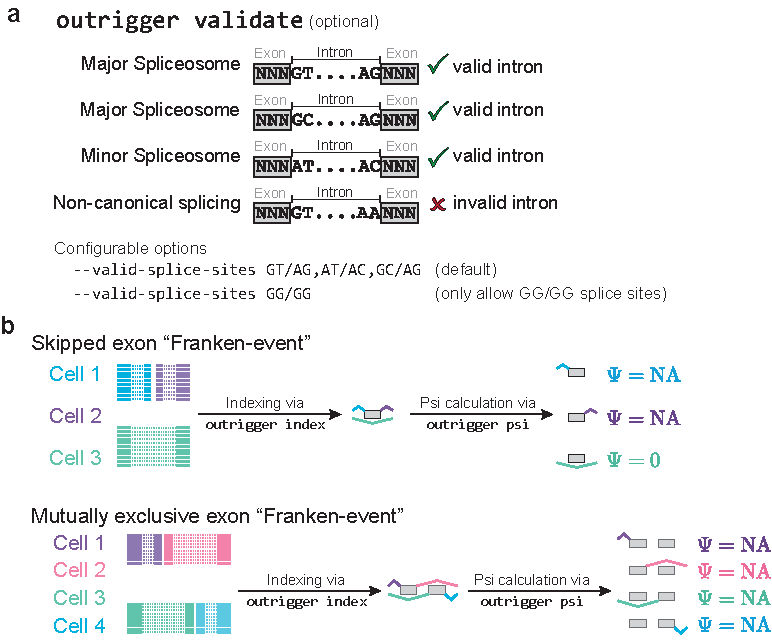
\includegraphics[width=5.8in]{figures/outrigger_validate}
  \caption[\outrigger\, validation and pathological cases.]{
  \outrigger\, validation and pathological cases.\\
\textbf{a.}~Validation via \texttt{outrigger validate}: Removal of alternative events with introns lacking consensus splice sites. In this optional step, exons with flanking introns lacking known splice site motifs are removed. This is configurable. By default, the valid splice sites are specified as, \texttt{-{}-valid-splice-sites GT/AG,GC/AG,AT/AC}, but can be any pair of two nucleotides.\\
\textbf{b.}~Possible pathological cases of \texttt{outrigger}. These ``Franken-events'' consist of junctions that were observed in independent samples. At the indexing step, aggregated reads from multiple cells/samples are considered to construct an index of all junctions to maximize the number of AS events. Yet, at the Psi/$\Psi$ calculation step, in each individual cell/sample, insufficient reads may be observed for certain junction resulting in $\Psi=\text{NA}$ in some cells/samples for the same event. Top, skipped exons, if each junction is observed only in one cell, the cell with the exclusion junction is assigned a $\Psi=0$ while the remaining cells are assigned as $\Psi=\text{NA}$. Bottom, mutually exclusive exons, $\Psi=\text{NA}$ for all 4 cells, as there is insufficient evidence of exon inclusion or exclusion in any one cell. Thus, the number of detected events output by \texttt{outrigger index} can greatly overestimate the number of valid events in the dataset found by \texttt{outrigger psi}.
}
\label{fig:outrigger_validate_frankenevents}
\end{figure}



\paragraph{\texttt{outrigger psi}: Calculate percent spliced-in of alternative exons}

To calculate percent spliced-in (Psi/$\Psi$) of a potentially alternative exon identified in \texttt{outrigger index}, we use the equation for $\Psi= \frac{\text{inclusion reads}}{\text{total reads}}$ \cite{Wang2008-xh}, with substantial checks for whether the event is valid (\textbf{\Cref{fig:outrigger_psi}}). For SE, there is only one exclusion junction and thus the the exclusion junction is weighted by two to compensate (Eq.~\Cref{eq:se_psi}). For MXE, the calcluation is simply the inclusion reads divided by the total reads (Eq.~\Cref{eq:mxe_psi}). The junction reads between exon $i$ and exon $j$ are presented as $r_{i,j}$, displaying inclusion reads in red and exclusion reads in blue.

\begin{multicols}{2}
\noindent
  \begin{gather}
  \text{SE $\Psi$}\nonumber\\
\Psi = \frac{\textcolor{inclusion}{r_{1,2}} + \textcolor{inclusion}{r_{2,3}}}{\textcolor{inclusion}{r_{1,2}} + \textcolor{inclusion}{r_{2,3}} + 2\textcolor{exclusion}{r_{1,3}}} \label{eq:se_psi} %\nonumber
\end{gather}
% \break
\begin{gather}
  \text{MXE $\Psi$}\nonumber\\
\Psi = \frac{\textcolor{inclusion}{r_{1,2}} + \textcolor{inclusion}{r_{2,4}}}{\textcolor{inclusion}{r_{1,2}} + \textcolor{inclusion}{r_{2,4}} + \textcolor{exclusion}{r_{1,3}} + \textcolor{exclusion}{r_{3,4}}} \label{eq:mxe_psi} %\nonumber
\end{gather}
\end{multicols}

Multiple validation steps were incorporated to ensure that the junction reads observed in each sample are consistent with the type of splicing event annotated by \outrigger. This process is described in \textbf{Supplementary Software .~\Cref{fig:outrigger_psi}}.

% --- BEGIN manual facingcaption --- %
\clearpage
\thispagestyle{facingcaption}
\begin{figure}[h]
\captionsetup{labelformat=prev-page}
  \caption[Cases created by percent spliced-in calculation via the command \texttt{outrigger psi}.]{
  Cases created by percent spliced-in calculation via the command \texttt{outrigger psi}.\\
% \captionof{figure}{\textbf{}
The table describes the 11-step sequential logic of \outrigger\, to reject an event in a cell/sample based on that cell/sample's junction reads. If an event reaches a $\Psi=\text{NA}$ case, then it is rejected from that sample, otherwise, it continues through the cases. If the event is rejected, then it is assigned $\Psi = \text{NA}$, if it is not rejected, then it gets a $0\leq \Psi \leq 1$ value based on the junction reads.\\
Strict evaluation of percent spliced-in (Psi/$\Psi$). To compute the percent spliced-in (Psi/$\Psi$) of skipped exon (SE) and mutually exclusive exons (MXE) alternative events during the execution of the command \texttt{outrigger psi}, we use $\Psi= \frac{\text{inclusion reads}}{\text{total reads}}$. We represent the number of reads spanning the junction between exon$_i$ and exon$_j$ as $r_{i,j}$.
}
\label{fig:outrigger_psi}

\end{figure}
\clearpage
\begin{figure}[h]
\ContinuedFloat
\captionsetup{labelformat=empty}
\centering
% \includegraphics[width=5.8in]{sandiego.jpg}
  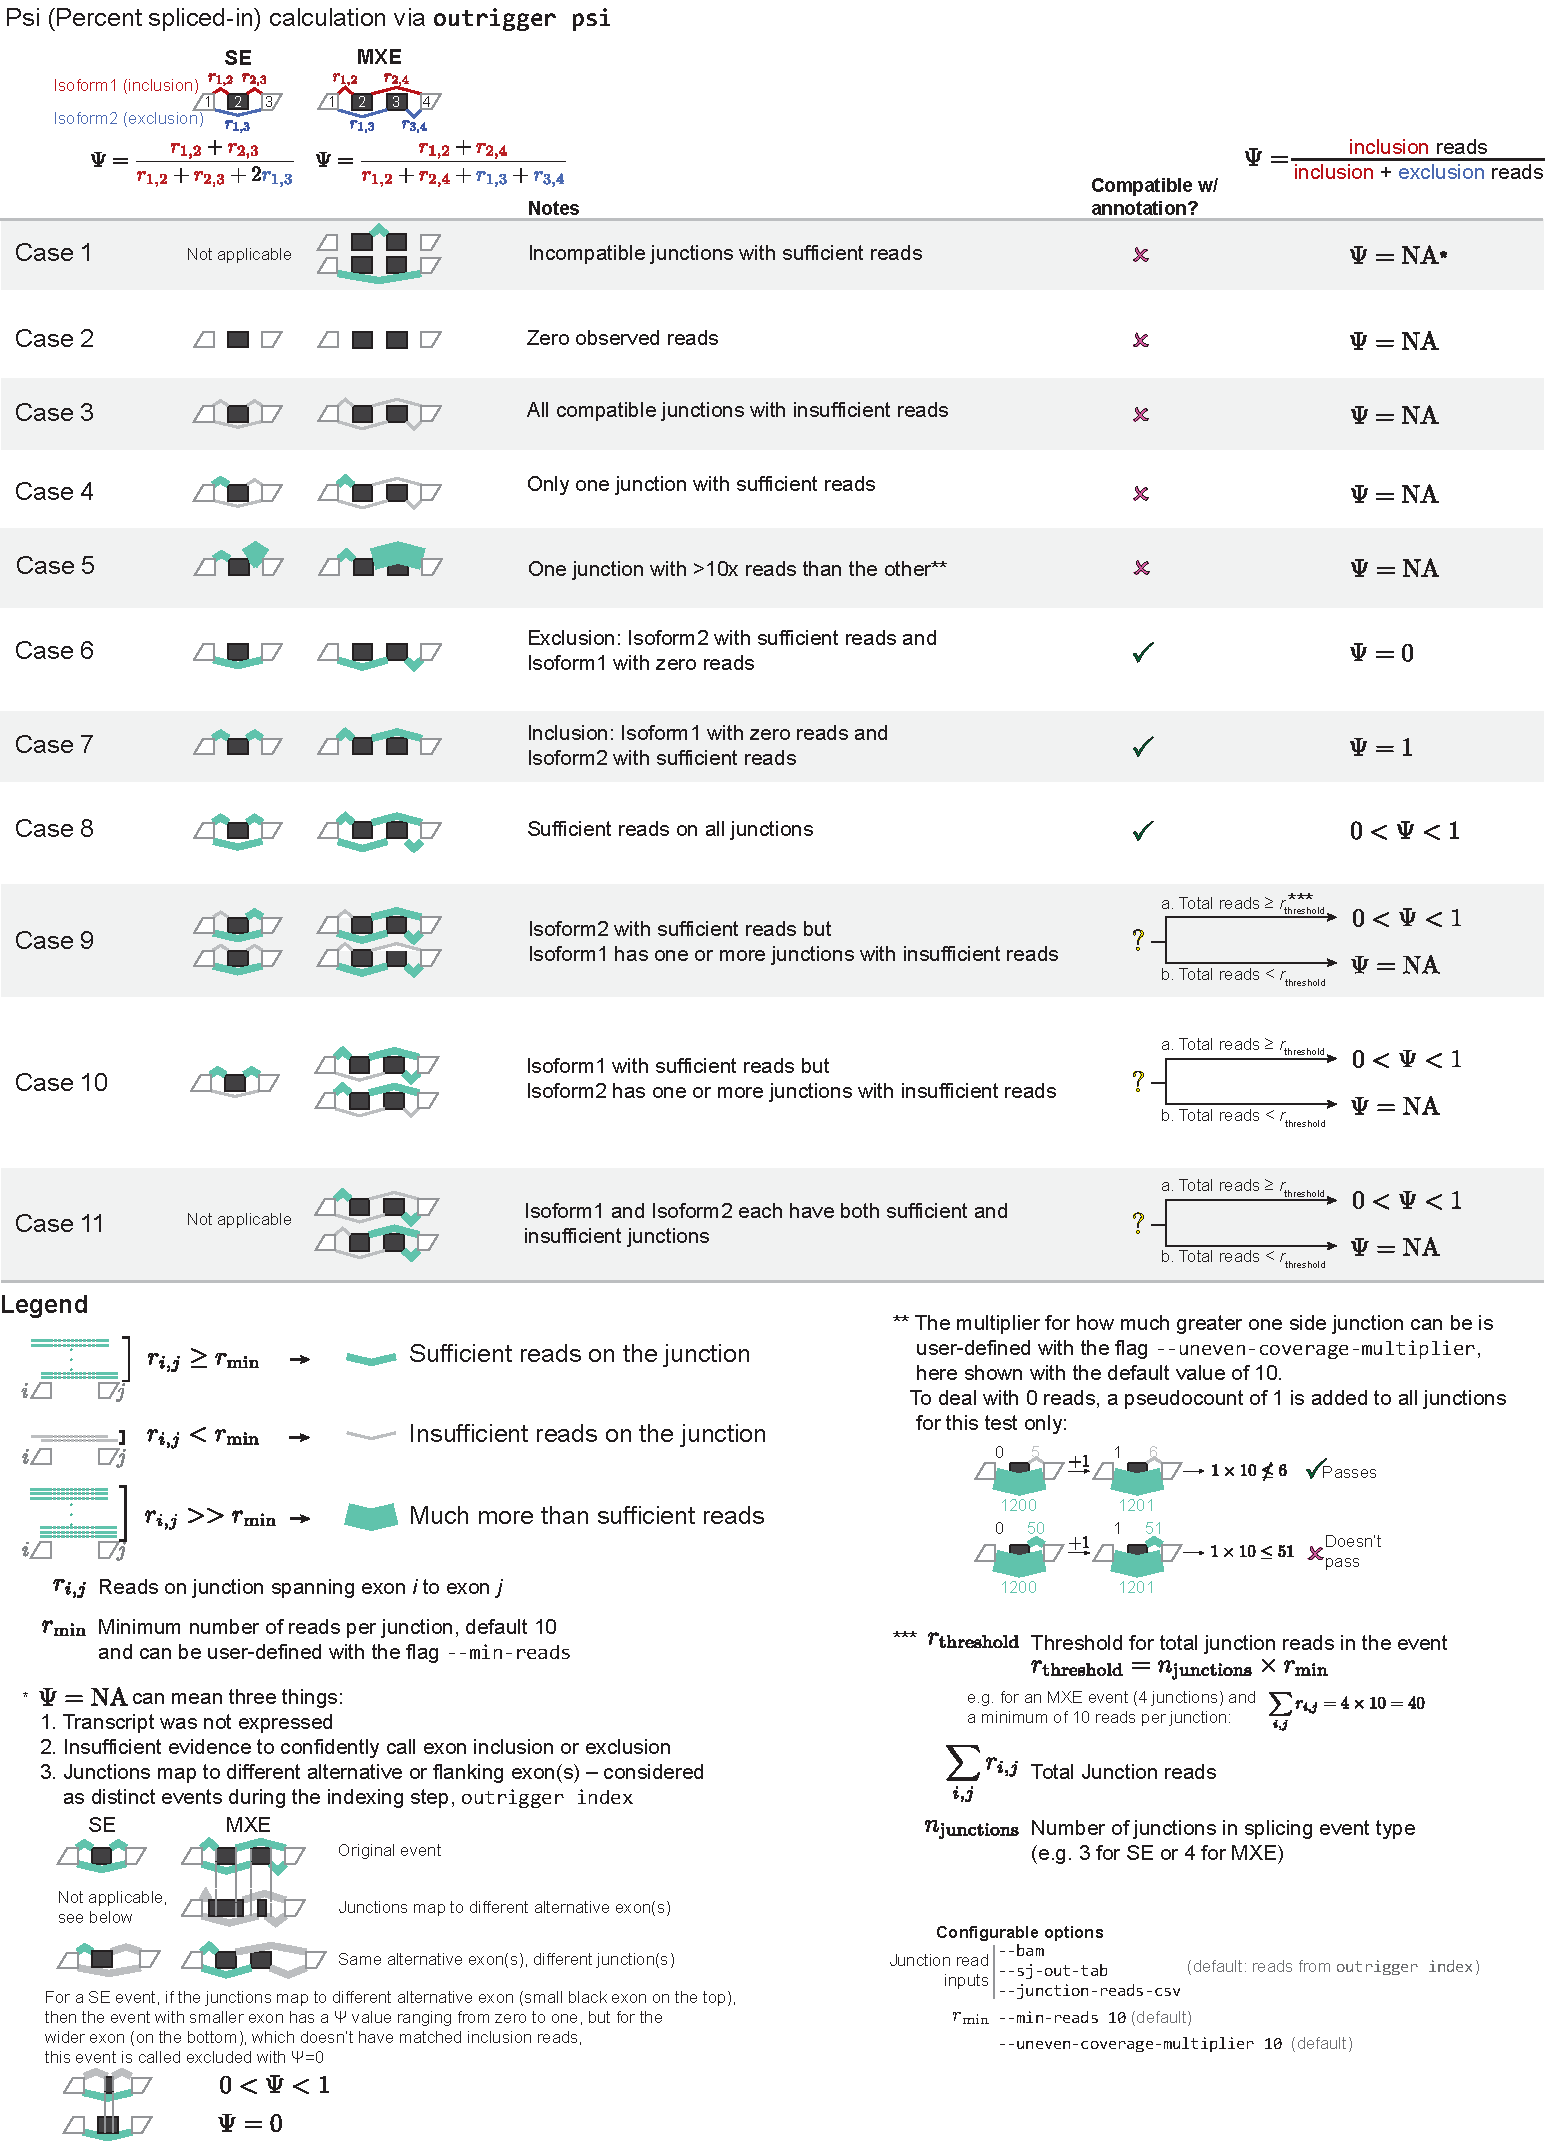
\includegraphics[width=5.8in]{figures/outrigger_psi}
\end{figure}
%and, I'm not sure why, but one of the times I used this code the figure number wasn't augmented for the next figure, so check your figure numbers and if necessary uncomment the following line
\addtocounter{figure}{1}
\clearpage
% --- END manual facingcaption --- %

\begin{longdescription}
	\item[Case 1: Incompatible junctions with sufficient reads.] This step checks whether the junction reads are compatible with a MXE event, or rather a twin cassette event. Specifically, evidence of  $r_{2,3} > r_{\min}$ or $r_{1,4} > r_{\min}$ suggests this junction is a twin cassette event but not an MXE event. In such cases, $\Psi = \text{NA}$. As described in \texttt{outrigger index}, the minimum number of reads is user-defined, for example to 37 with \texttt{-{}-min-reads~37}.
	\item[Case 2: Zero observed reads.] Given no reads is observed, this event is $\Psi = \text{NA}$, rather than $\Psi=0$ since $\Psi=0$ indicates exclusion.
	\item[Case 3: All compatible junctions with insufficient reads.] No single junction has the minimum number of reads $r_{\min}$, by default $r_{\min}$ is 10, and can be modifiable by the \texttt{-{}-min-reads} flag. If this is the case, we assign $\Psi = \text{NA}$.
	\item[Case 4: Only one junction with sufficient reads.] This applies to a single junction of two junctions per isoform, e.g. Isoform2 of either SE or MXE events, and Isoform1 of an MXE event, has sufficient reads. Since only one junction has the minimum number of reads, $r_{\min}$, no sufficient evidence indicates inclusion of exon-of-interest, thus, we assign $\Psi = \text{NA}$.
	\item[Case 5: One junction with $>10\times$ more reads than the other.] When the alternative exon is covered on the two sides with junction reads of great disparity, there is insufficient evidence supporting the inclusion of alternative exon or suggests the exon may involved in a complex splicing, rather than a SE or MXE. Thus, $\Psi = \text{NA}$. The default multiplier is 10 and can be modified by the user, for example to 55 by \texttt{-{}-uneven-coverage-multiplier~55}.
	\item[Case 6: Exclusion: Isoform2 with sufficient reads and Isoform1 with zero reads.] All junctions on Isoform2 have greater than the minimum reads $r_{\min}$, and all junctions of Isoform1 have no observed reads, thus $\Psi = 0$.
	\item[Case 7: Inclusion: Isoform2 with zero reads and Isoform1 with sufficient reads.] All junctions on Isoform2 have no observed reads and all junctions of Isoform1 have greater than the minimum reads $r_{\min}$, thus $\Psi = 1$.
	\item[Case 8: Sufficient reads on all junctions.] Both Isoform1 and Isoform2 have greater than the minimum reads on all their junctions. This is the best possible case for alternative splicing.
	\item[Case 9: Isoform2 with sufficient reads but Isoform1 has one or more junctions with insufficient reads.] If the exclusion isoform, Isoform2 has sufficient reads, but the inclusion isoform (Isoform1) does not, then we assess whether the total read coverage of the event, $\sum_{i,j} r_{i,j}$exceeds $r_{\text{threshold}}$. If so, a $\Psi$ is calculated; if not, $\Psi = \text{NA}$. We define $r_{\text{threshold}}$ as the number of junctions $n$ times the minimum number of reads $r_{\min}$. For example, with a minimum read count is 10 on an SE event, $r_{\text{threshold}} = 30$. For a minimum read count of 10 on an MXE event, $r_{\text{threshold}} = 40$.
	\item[Case 10: Isoform2 has one or more junctions with insufficient reads but Isoform1 has sufficient reads.] Similar to Case 9, we again test if the total read coverage is sufficient to calculate $\Psi$, i.e. if $\sum_{i,j} r_{i,j} \geq r_{\text{threshold}}$. If so, we calculate $\Psi$, and if not, we assign $\Psi = \text{NA}$.
	\item[Case 11: Isoform1 and Isoform2 each have both sufficient and insufficient junctions.] This case only applies to MXE events as SE events have as single Isoform2 junction, and cannot have both sufficient and insufficient junctions. If by the per-junction coverage, it is unclear whether the event has sufficient coverage, then we test if the total coverage of the event is sufficient. If so, we calculate $\Psi$, and if not, we assign $\Psi = \text{NA}$.
\end{longdescription}


% Before we calculate $\Psi$, we ensure that a sample has a valid SE event by checking for enough reads on either both the inclusion junctions ($r_{1,2}$ and $r_{2,3}$) or the exclusion junction ($r_{1,3}$). This protects against calculating $\Psi$ for events that aren't truly SE or MXE events, for example, an alternative first exon event that was annotated as an SE event would have $r_{1,2} = 0$, and thus we wouldn't calculate $\Psi$. For MXE events, we check that there are no reads between exons 2 and 3 ($r_{2,3}=0$), because if there are any reads here, then this is evidence that in a particular sample, this is a twin casette event rather than an MXE event (\textbf{Supplementary \Cref{fig:outrigger_psi}}). For SE events, we also check that for inclusion, there must be $>10$ reads on both sides of the alternative exon, and if there aren't, then we discard the event.
\subparagraph{Outputs} The output of \texttt{outrigger psi} is added into the \\\texttt{outrigger\_output} folder by creating a \texttt{psi} folder for each splice type. \texttt{psi.csv} contains $\Psi$ in a matrix, and the \texttt{summary.csv} produces a summary of all the events observed in all samples with their junction reads.

To follow up with our \texttt{outrigger index} and \texttt{outrigger validate} commands, we can run the below example command in the same directory:

\begin{verbatim}
outrigger psi
\end{verbatim}

This command adds to the existing output folder \texttt{outrigger\_output}. Therefore, we don't need to specify a genome location or reads or index location if this command is run from the same folder as the \texttt{outrigger index} command was run, and there exists in the directory a folder called \texttt{outrigger\_output}.

\begin{figure}
\footnotesize
\dirtree{%
.1 outrigger\_output/.
.2 index.
.3 gtf.
.4 gencode.vM10.annotation.gtf.
.4 gencode.vM10.annotation.gtf.db.
.4 novel\_exons.gtf.
.3 exon\_direction\_junction.csv.
.3 mxe.
.4 event.bed.
.4 events.csv.
.4 exon1.bed.
.4 exon2.bed.
.4 exon3.bed.
.4 exon4.bed.
.4 intron.bed.
.4 splice\_sites.csv.
.4 validated.
.5 events.csv.
.3 se.
.4 event.bed.
.4 events.csv.
.4 exon1.bed.
.4 exon2.bed.
.4 exon3.bed.
.4 intron.bed.
.4 splice\_sites.csv.
.4 validated.
.5 events.csv.
.2 junctions.
.3 metadata.csv.
.3 reads.csv.
.2 psi.\DTcomment{Added by \texttt{outrigger psi}}.
.3 mxe\DTcomment{Added by \texttt{outrigger psi}}.
.4 psi.csv\DTcomment{Added by \texttt{outrigger psi}}.
.4 summary.csv\DTcomment{Added by \texttt{outrigger psi}}.
.3 outrigger\_psi.csv\DTcomment{Added by \texttt{outrigger psi}}.
.3 se\DTcomment{Added by \texttt{outrigger psi}}.
.4 psi.csv\DTcomment{Added by \texttt{outrigger psi}}.
.4 summary.csv\DTcomment{Added by \texttt{outrigger psi}}.
}
\caption{Example output of \texttt{outrigger psi} command.}
\end{figure}

\paragraph{Advantages and limitations of \outrigger.}

The main advantages of \outrigger\, are speed and conserved memory footprint. As \outrigger\, operates only on junction reads, rather than resampling reads from a \texttt{.bam} alignment file, which can range in size from 500MB to 20GB and results in a high memory footprint, \texttt{outrigger} summarizes each \texttt{.bam} file to only its junction reads and uses that to estimate Psi/$\Psi$ values. Additionally, employing three steps of \outrigger\, \outrigger\ is able to maximize the number of potential alternative events and subsequently apply strict validation rules in the step of outrigger psi calculation to eliminate false positive events from each sample.
However, currently, \outrigger\ can only deal with SE and MXE events. We are in the process of incorporating other alternative splice types.

% \subsection{PCR duplicate removal studies}

% We also compared outrigger's performance on pre- and post-duplicate removed dataset. After duplicate-removal, ~93\% events were retained by requiring that each junction is covered by at least 10 unique reads (\textbf{Supplementary \Cref{fig:splicing_qc}f}). When comparing the Psi scores before and after duplicate-removal, the vast majority of events have a consistent Psi within |delta Psi| < 0.2 and only ~7\% are designated as NA in the latter (\textbf{Supplementary \Cref{fig:splicing_qc}h-i}), likely due to the reduced read coverage.

\subsection{Comparison to other methods}

In comparison to the popular splicing program MISO\cite{Katz:2010iv}, \outrigger\, has three major advantages:

\begin{enumerate}
	\item Ability to build de novo exon indexes (\texttt{outrigger index})
	\item Flexiblity of junction-based definitions of alternative exons, enumerating all possible flanking exons (\texttt{outrigger index})
	\item Ability to eliminate incompatible alternative events (\texttt{outrigger psi})
	\item Speed of evaluation. Instead of using the huge \texttt{.bam} alignment files directly, \outrigger\, summarizes the files as junction reads, leading to much faster calculation of percent spliced-in. Once an index is built with \texttt{outrigger index} (24-48 hours), then calculation of $\Psi$/Psi takes 2-4 hours, even on hundreds of samples. With MISO, the calculation can take 8 hours per sample.
\end{enumerate}


\paragraph{Ability to build de novo exon indexes.} MISO provides pre-built alternative splicing indexes, which may not be incompatible with the data at hand. There is a program, GESS \cite{Ye:2014cd} to detect alternative exons from \texttt{.bam} files, which can only handle a handful files at a time and freeze when given hundreds of single-cell \texttt{.bam} files. In contrast, in the outrigger indexing step, \outrigger\,builds indexes based on provided data, which will be integrated with provided exon annotation allowing identification of novel exons.

\paragraph{Flexiblity of junction-based definitions of alternative exons, enumerating all possible flanking exons.} Multiple possible flanking exons can be associated with an alternative exon, most algorithms, including MISO and rMATS \cite{Shen2014-zq}, choose a single set (often the shortest one), rather than being flexible and allowing the user to choose the relevant ones. The resulting ``best guess'' of the alternative event may not be biologically relavent and may be misleading to interprete. In such case, computational translation of alternative events, as demonstrated in Figure 4, will not be possible.

\paragraph{Ability to eliminate incompatible alternative events} Comparing MISO $\Psi$ values side-by-side with a corresponding \texttt{outrigger psi} calculation, we find that $46\%$ of MISO $\Psi$ values are rejected and assigned $\Psi = \text{NA}$ by \outrigger\, (\textbf{\Cref{fig:miso}}).

A large group of false positives that are correctly rejected by \outrigger\, are Case 1, where only incompatible junctions present sufficient reads. For example, when twin cassette events are annotated as MXE events and the data indicates inclusion of both alternative exons, MISO will calculate $\Psi$ as 0.5. Because MISO uses a prior of $\Psi=0.5$ and resamples the data to calculate $\Psi$. In such a case, MISO is never convinced that $\Psi$ should be towards 1 or 0 and remains at $\Psi~0.5$ (\textbf{\Cref{fig:miso}a}). %As a result, these false positive MXE events make up a far larger proportion of the middle modality when using MISO data than with \outrigger\, (\textbf{\Cref{fig:miso}e-f}).

% --- BEGIN manual facingcaption for MISO figure --- %
\clearpage
\thispagestyle{facingcaption}
\begin{figure}[h]
\captionsetup{labelformat=prev-page}
  \caption[Examples of inconsistencies in MISO's estimation with single-cell data.]{Examples of inconsistencies in MISO's estimation with single-cell data.\\
\textbf{a-c}. Representative examples of SE and MXE AS events measured by MISO, but were unsupported with visual inspection on IGV browser, and were disqualified by \outrigger. To identify SE and MXE events, \outrigger\, constructs a \emph{de novo} splicing index based on the junction reads in all libraries in the dataset (see details in \textbf{Figures~\cref{fig:outrigger_index,fig:outrigger_psi,fig:outrigger_validate_frankenevents}}). The following examples are not considered by \outrigger as true SE or MXE events, therefore annotated as NA. Note, MISO does not estimate modality for each event, \anchor\, (see details in \textbf{\Cref{fig:anchor_overview,fig:anchor_simulations_perfect_modalities,fig:anchor_simulations_maybe_bimodals}}) was used to estimate modality.\\
\textbf{a.} Top, a MISO-annotated MXE event in ARF4 with MISO estimated $\Psi$s $\sim0.5$ and classified as ``middle'' modality in each of iPSC, NPC, and MN by \anchor. Yet, in the IGV browser (bottom), this event appears as a twin cassette event, where both exons 2 and 3 are included, indicating that at least in our dataset this event is not consistent with the MISO annotation. Outrigger disqualifies this event as a MXE and assign NA (top left).\\
\textbf{b.} Top, a MISO-annotated SE event in CLF1 with MISO estimated $\Psi$s ranging from $0.1$ to $0.6$ and is classified as a ``middle'' modality event by \anchor\, in each of iPSC, NPC, and MN.  Yet, in the IGV browser (bottom), exon 1 for this annotation is not covered at all. Given the data, outrigger\ do not consider this as a bona fide SE event and assign NA to this event.\\
\textbf{c.} Top, a MISO-annotated MXE event in AHSA1 with a wide range of MISO calculated $\Psi$s and is classified as the ``multimodal'' modality in each of iPSCs, NPC, and MN populations by \anchor. Bottom, in the IGV browser. Exons 2 and 3 are the annotated alternative exons for MXE, however, another two well-covered exons between exon 2 and 3 were observed and one extra exon between exon 3 and 4, which disqualify this event as an MXE event. Furthermore, when both exon 2 and 3 are included, MISO estimated $\Psi$ scores are closer to 1 instead of around $0.5$, as was seen in (\textbf{a}). Thus, outrigger rejects this as MXE and assign NA.\\
\textbf{d.}~Using \outrigger\,'s strict rules on MISO annotations, the majority (51\%) of the data generated by MISO was rejected by \outrigger\, (left). Right, using the exact same annotation from MISO, \outrigger\, 22\% of events found by \outrigger\, had too wide of a confidence interval ($>0.4$) by MISO.\\
\textbf{e.}~Heatmap comparing the numbers and percentages of alternative events that were within $|\Delta\Psi| < 0.2$, switched to exactly 1 or 0 in \outrigger, were NA in either MISO or \outrigger, or were in another case.\\
\textbf{f.}~Barplot of the number of cases found only in MISO (orange) and rejected as NA by \outrigger, and of the cases found only by \outrigger (green) and considered to have too wide of a confidence interval by MISO.\\
To summarize, \texttt{outrigger} follows strict rules to identify alternative splicing (\textbf{Figures~\cref{fig:outrigger_index,fig:outrigger_psi,fig:outrigger_validate_frankenevents}}) and provides a $\Psi$ distribution more localized at the extremes of $\Psi = 0$ and $\Psi = 1$. Although \texttt{outrigger}, may identify fewer events, they are true SE and MXE events.}
\label{fig:miso}
\end{figure}
\clearpage
\begin{figure}[h]
\ContinuedFloat
\captionsetup{labelformat=empty}
\centering
% \includegraphics[width=5.8in]{sandiego.jpg}
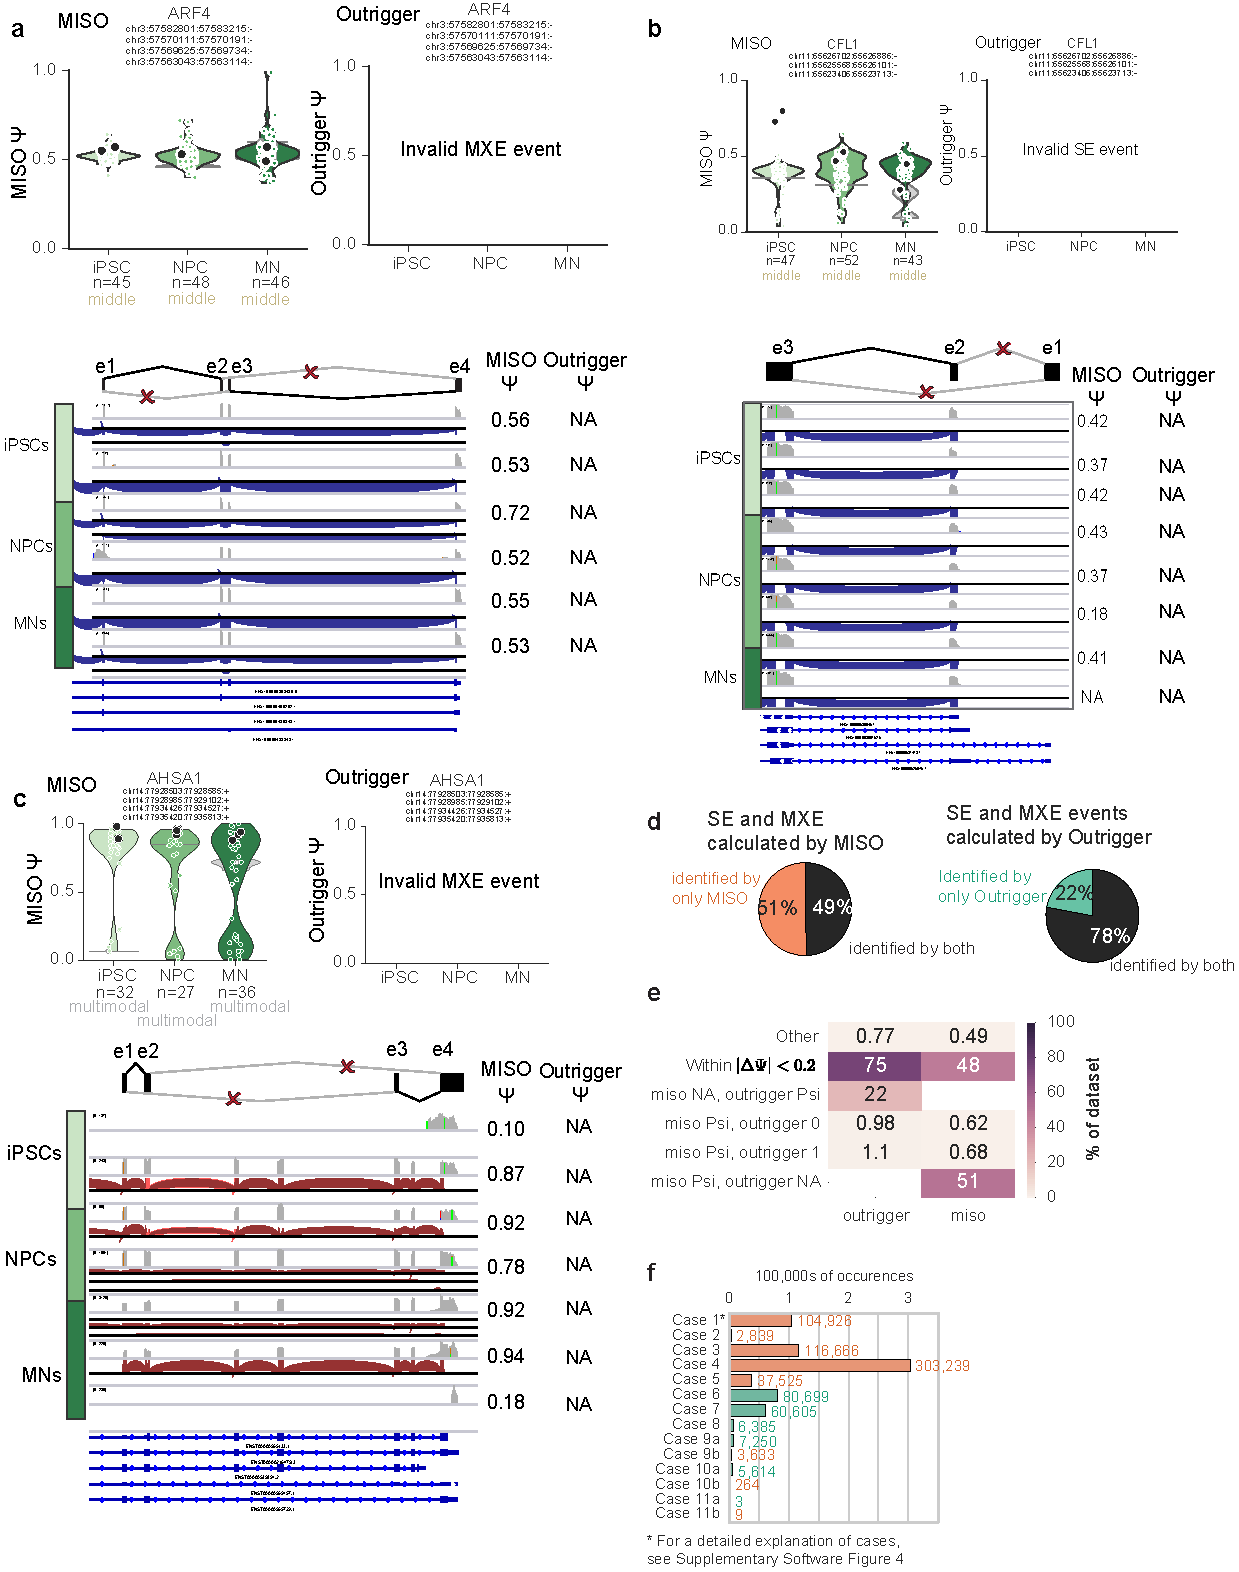
\includegraphics[width=5.8in]{figures/invalid_miso.pdf}
\end{figure}
%and, I'm not sure why, but one of the times I used this code the figure number wasn't augmented for the next figure, so check your figure numbers and if necessary uncomment the following line
%\addtocounter{figure}{1}
\clearpage
% --- END manual facingcaption for MISO fiugre --- %


The majority of the false positives are Case 4, where only one junction has sufficient reads. As MISO counts both junctions to calculate $\Psi$, shown in \textbf{\Cref{fig:miso}b-c}, many of the events are not covered on both sides of the alternative exons, which may suggest the events are not true SE events, but rather alternative first exon events, for instance.

We used MISO's event definitions and found that as many as 50\% of MISO events did not pass the stringent rules of \outrigger, primarily due to the incompatibility with the annotation of SE and MXE and insufficient coverage (\textbf{\Cref{fig:miso}j-l}).


\section{\texttt{anchor}: Modality estimation}
\label{sec:anchor}

\subsection{Algorithm overview}
\paragraph{Model modalities as beta distributions}

% \theoremstyle{definition}
We define \emph{modality} as a distinct type of distributions. Since $\Psi$s are continuous value between $(0, 1)$, distribution of $\Psi$ can be modeled as Beta distribution. The probability density function for the Beta distribution, $\mathrm{Pr}(\alpha, \beta)$ is defined between $(0, 1)$, with parameters $\alpha > 0$ and $\beta > 0$,

\begin{equation}
\mathrm{Pr}(\alpha, \beta) \sim \frac{1}{\mathrm{B}\left(\alpha, \beta\right)}  x^{(\alpha - 1)} \left(1-x\right)^{(\beta-1)},
\end{equation}

where $\mathrm{B}\left(\alpha, \beta\right)$ is the Beta function, defined by $\alpha > 0$ and $\beta > 0$. It may be easier to think about how the $\alpha$ and $\beta$ parameters affect distribution by observing the mean and variance \textbf{\Cref{fig:anchor_parameterization}a}. The beta distributions can be described by four parameterizations: $1 \leq \alpha < \beta$, $\alpha = \beta > 1$, $\alpha > \beta \geq 1$, $\alpha = \beta < 1$ (\textbf{\Cref{fig:anchor_parameterization}b}). Conveniently, these four configurations correspond to the four modalities we are interested in: $1 \leq \alpha < \beta$ corresponds to \emph{excluded}, $\alpha = \beta > 1$ to \emph{middle}, $\alpha > \beta \geq 1$ to \emph{included}, and $\alpha = \beta < 1$ to \emph{bimodal} (\textbf{\Cref{fig:anchor_parameterization}c}). The final \emph{multimodal} modality corresponds to $\alpha = \beta = 1$, which is equivalent to the uniform distribution used as null model.



\paragraph{Model parameterization}
To describe feature distribution as modalities, we parameterized the four parameterizable modalities and used Bayesian model selection to choose the best model to describe the distribution. Python package \texttt{scipy}\cite{Oliphant:2007dm,Millman:2011jv} was used to implement Beta distribution.
For \1 (\0) modality, we fixed $\beta$ ($\alpha$) at 1 and linearly increased $\alpha$ ($\beta$) from $2$ to $20$ (\Cref{fig:anchor_parameterization}d). We chose $2$ as a starting parameter since it is near the $\alpha=\beta=1$ uniform distribution, as we wanted to allow \0 and \1 distributions with noise. For bimodal (middle) modality, we changed $\alpha$ and $\beta$ simultaneously, monotonically decreasing (increasing) the parameters from $\alpha=\frac{1}{12}$, $\beta = \frac{1}{12}$ ($\alpha = 2, \beta = 2$) to $\alpha = \frac{1}{30}, \beta = \frac{1}{30}$ ($\alpha = 20, \beta=20$). The parameters for bimodal start at $\frac{1}{12}$ rather than $\frac{1}{2}$ because starting the parameters from $\frac{1}{2}$ resulted in more false positive ``bimodal'' events, whereas starting the parameters from $\frac{1}{2}$ ensures any density near $0.5$ is downweighted.


The fit of feature distribution is assessed to the four configurations using Bayes Factors, represented by $K$,

\begin{align}
K^{(m)}
&= \frac{P(D | M_1^{(m)})}{P(D | M_0)}\\
&=
\frac{\sum_{i} P(\alpha_i^{(m)}, \beta_i^{(m)} | M_i^{(m)}) P(D | \alpha_i^{(m)}, \beta_i^{(m)}, M_i^{(m)})}
{\sum P(\alpha_0, \beta_0 | M_0) P(D | \alpha_0, \beta_0, M_0)}\\
&=
\frac{\sum_{i} P(\alpha_i^{(m)}, \beta_i^{(m)} | M_i^{(m)}) P(D | \alpha_i^{(m)}, \beta_i^{(m)}, M_i^{(m)})}
{1}\\
&=
\sum_{i} P(\alpha_i^{(m)}, \beta_i^{(m)} | M_i^{(m)}) P(D | \alpha_i^{(m)}, \beta_i^{(m)}, M_i^{(m)})
\end{align}

Where $M_i^{(m)}$ is the model of interest (e.g. $M_i^{(\mathrm{bimodal})}$) and $\alpha_i^{(m)}, \beta_i^{(m)}$ are the corresponding parameters from the parameterization shown in \textbf{\Cref{fig:anchor_parameterization}d}. The null model, $M_0$ is the uniform distribution, where $\alpha_0 = \beta_0 = 1$, and thus $P(D|M_0) = 1$ for all datasets. We use a Bayes Factor cutoff of $K_{\mathrm{cutoff}}$ to indicate the threshold where the model begins to explain the data reasonably well. In practice we set $K_{\mathrm{cutoff}} = 2^{5}$ ($\log_2 K_\mathrm{cutoff} = 5$).

The \0 and \1 modalities vary only one parameter at a time, whereas middle and bimodal modalities vary both $\alpha$ and $\beta$ simoutanously. Models with more parameters are more likely to fit, thus we fit to the one-parameter models first, assessing whether $K > K_{\mathrm{cutoff}}$ for either \0 or \1. No distribution can fit both \0 and \1 modalities, thus it is assigned to the modality with highest $K$. Next, the distribution is fitted to the two-parameter bimodal and middle models, checking if $K > K_{\mathrm{cutoff}}$. If neither modality applies, we assign the modality to \emph{multimodal} (\textbf{2c}).

% --- BEGIN manual facingcaption for anchor_parameterization --- %
\clearpage
\thispagestyle{facingcaption}
\begin{figure}[h]
\captionsetup{labelformat=prev-page}
  \caption[Overview of \anchor\, parameterization of the Beta distribution.]{
  Overview of \anchor\, parameterization of the Beta distribution.\\
\textbf{a.}~Top, equation for the Beta distribution of the random variable $x$ with parameters $\alpha, \beta > 0$. Bottom left, equation for the mean ($\mu$) of the Beta distribution as a function of its parameters. Bottom right, equation for the variance ($\sigma^2$) of the Beta distribution as a function of parameters.\\
\textbf{b.}~Cartoon of valid values of $\alpha$ and $\beta$ parameters of Beta distribution, showing how the space is partitioned by the modalities.\\
\textbf{c.}~Violinplots representing the four ideal modalities, plus the null ``multimodal'' distribution. Each modality is annotated with examples of four cells representing within-cell distributions of included (dark grey) and excluded (light grey) transcripts, and the corresponding parameters of the Beta distribution.\\
\textbf{d.}~Violinplots of 1 million random samples of the family of Beta distributions specified by the $\alpha$ and $\beta$ ($x$ tick labels) parameterization of the four modalities: excluded, bimodal, included, and middle.}
\label{fig:anchor_parameterization}
\end{figure}
\clearpage
\begin{figure}[h]
\ContinuedFloat
\captionsetup{labelformat=empty}
\centering
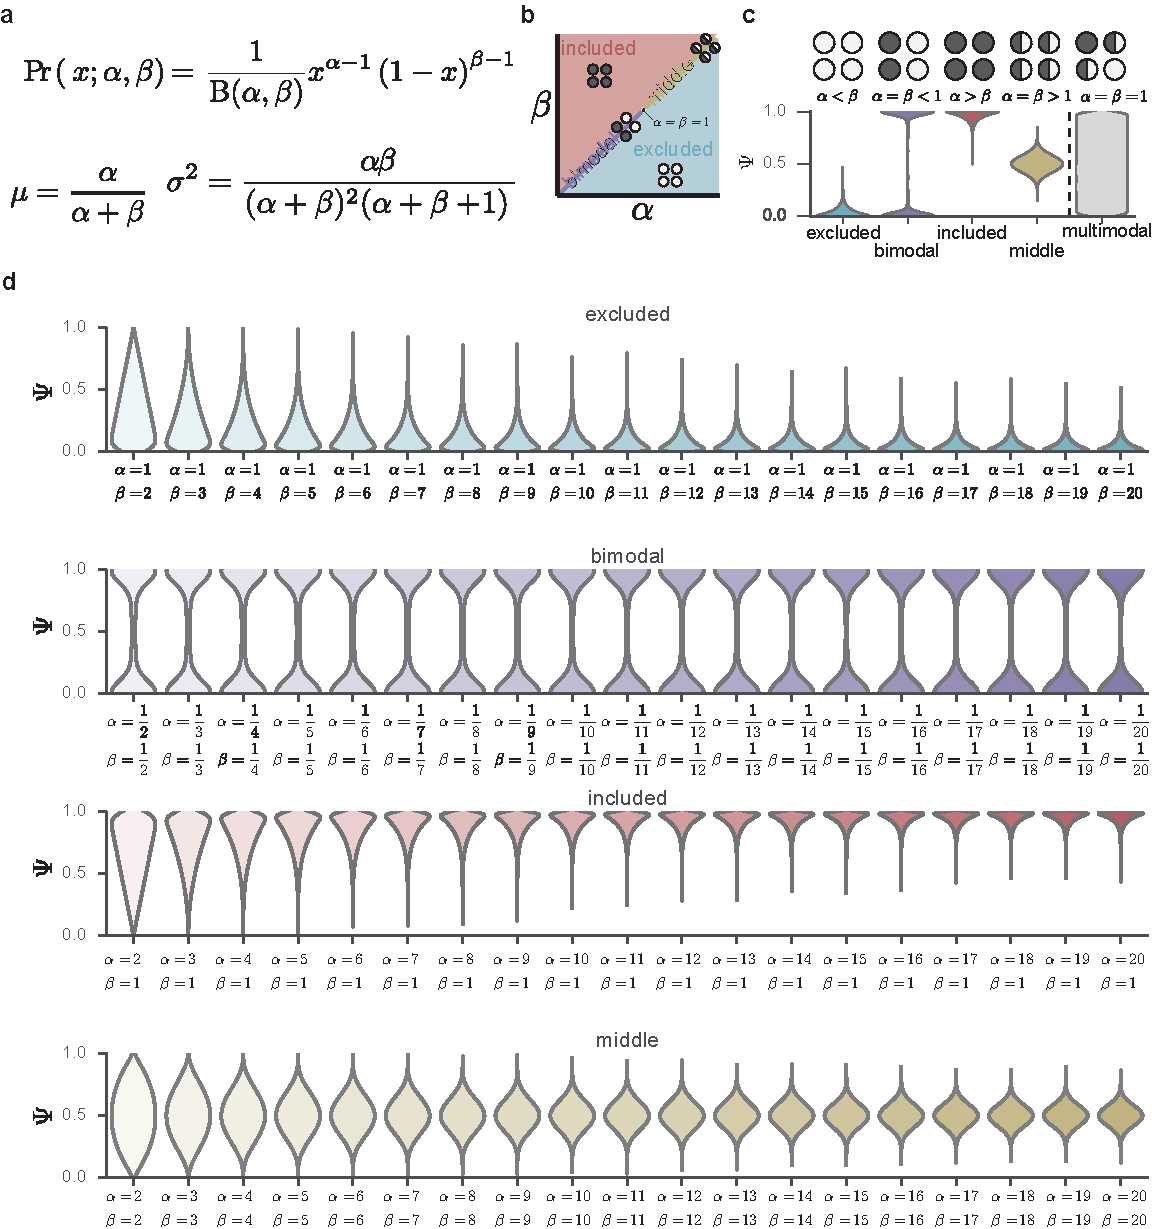
\includegraphics[width=5.8in]{figures/anchor_parameterization}
\end{figure}
%and, I'm not sure why, but one of the times I used this code the figure number wasn't augmented for the next figure, so check your figure numbers and if necessary uncomment the following line
\addtocounter{figure}{1}
\clearpage
% --- END manual facingcaption for anchor_parameterization --- %



As exact $0$ and $1$ are not in the range of the Beta distribution, we implement this model selection by adding a small number ($0.001$) to $0$ and subtracting this small number from $1$. Thus, we approximate the data-derived distribution from the invalid closed interval [0, 1] to the valid open interval of (0, 1).


\subsection{Simulations}

We optimized the algorithm parameters using test datasets and visually inspecting random samples from both the best- and worst-fitting data and ensuring that the even the worst fitting data was still believably categorized as the modality (\textbf{\Cref{fig:anchor_best_worst}}).

\paragraph{Dataset 1: ``Perfect Modalities'' with noise}
\label{sec:anchor_perfect_modalities}

To test the limits of \texttt{anchor}, we simulated perfectly \0, middle, \1, and bimodal distribution, added uniform random noise with 100 iterations, and estimated modality at each noise level with iteration (\textbf{\Cref{fig:anchor_simulations_perfect_modalities}a}). As expected, the most frequently predicted modality was ``multimodal,'' since the dataset was created from randomly added noise (\textbf{\Cref{fig:anchor_simulations_perfect_modalities}b}). The next frequent modality was bimodal, followed by a tie with excluded and included, and the least frequent one is middle modality. We found that these parameterizations can accurately predict modality with up to $35\%$ noise added to the middle modality, $50\%$ noise added to excluded and included modalities, and up to $70\%$ noise added to the bimodal modality(\textbf{\Cref{fig:anchor_simulations_perfect_modalities}d}). By visual inspection of distributions fit best or worst to each modality (\textbf{\Cref{fig:anchor_best_worst}a}), we observed that the bimodal distributions are sufficiently different from other parameterizations, demonstrating the robustness of the algorithm.



% --- BEGIN manual facingcaption for anchor best worst fits --- %
\clearpage
\thispagestyle{facingcaption}
\begin{figure}[h]
\captionsetup{labelformat=prev-page}
  \caption[Best and worst fitting modality data using \anchor.]{
  Best and worst fitting modality data using \anchor.\\
Left, 10 events with largest Bayes Factor, $K$ (best fit) from the assigned modality. Right, 10 events with smallest Bayes Factor, $K$ (worst fit) from their assigned modality. For multimodal, as there is no fit, this simply shows 20 random events.\\
\textbf{a.}~Bayesian \anchor\, method on ``Perfect modalities'' dataset.\\
\textbf{b.}~Bayesian \anchor\, method on ``Maybe bimodals'' dataset.
}
\label{fig:anchor_best_worst}
\end{figure}
\clearpage
\begin{figure}[h]
\ContinuedFloat
\captionsetup{labelformat=empty}
\centering
  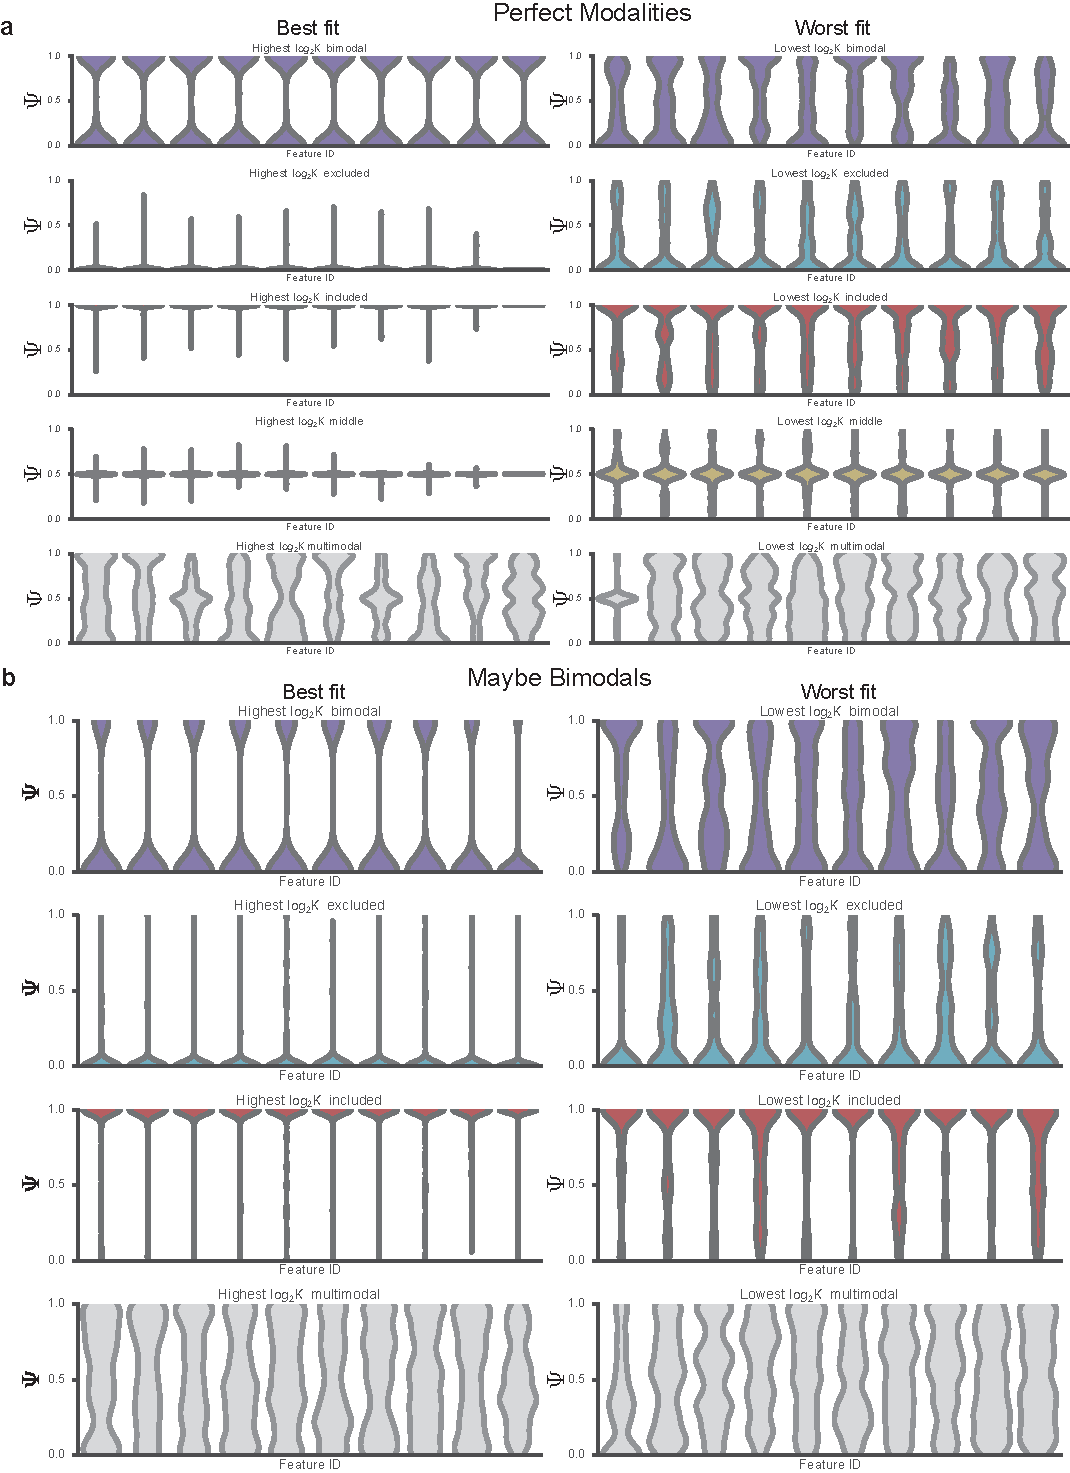
\includegraphics[width=5.8in]{figures/anchor_best_worst}
\end{figure}
%and, I'm not sure why, but one of the times I used this code the figure number wasn't augmented for the next figure, so check your figure numbers and if necessary uncomment the following line
\addtocounter{figure}{1}
\clearpage
% --- END manual facingcaption for anchor best worst fits --- %




% --- BEGIN manual facingcaption for perfect modalities anchor simulations --- %
\clearpage
\thispagestyle{facingcaption}
\begin{figure}[h]
\captionsetup{labelformat=prev-page}
\caption[Simulated ``Perfect Modality'' dataset to test performance of \texttt{anchor}.]{
Simulated dataset to test performance of \texttt{anchor}.\\
\textbf{a.}~Violinplots depicting the creation of simulated modality datasets with increasing noise. The base dataset (\% Noise = 0) consisted of 100 samples of either all zeros (excluded), half zeros and half ones (bimodal), all ones (included), or all $0.5$s (middle), exactly representing the four modalities. Uniform random noise was added in 5\% increments, with 100 iterations at each noise level.
\textbf{b.}~Percentage of events categorized as different modalities by \texttt{anchor} in the randomly generated test datasets, across all noise levels, as illustrated in (\textbf{a}). Number of events for each modality is annotated on top of the barplots. \\
\textbf{c.}~Percentage of events categorized as different modalities by binning in the randomly generated test datasets, across all noise levels, as illustrated in (\textbf{a}). Number of events for each modality is annotated on top of the barplots. \\
\textbf{d-g.}~Specificity of modality estimation. Recapitulation of the original modality as a function of additional noise, using \anchor\, (\textbf{d}), binning (\textbf{e}), Bimodality index (\textbf{f}), and diptest (\textbf{g}) methods. The $x$-axis depicts the percent of uniform random noise added (visualized as a triangle gradient), and the $y$-axis depicts the fraction of times a noisy feature was categorized into each modality. The hue of the line is the modality.
}
\label{fig:anchor_simulations_perfect_modalities}
\end{figure}
\clearpage
\begin{figure}[h]
\ContinuedFloat
\captionsetup{labelformat=empty}
\centering
% \includegraphics[width=5.8in]{sandiego.jpg}
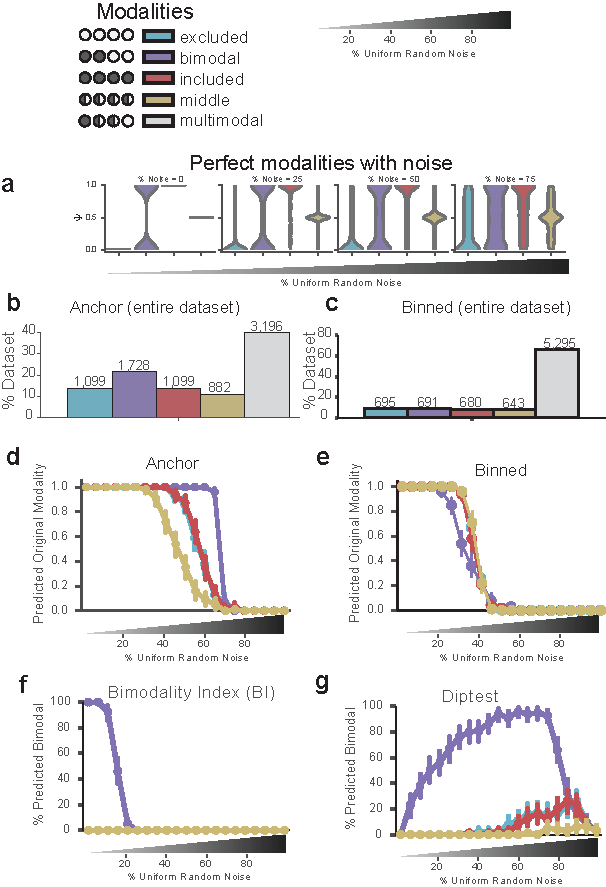
\includegraphics[width=5.8in]{figures/anchor_simulations_perfect_modalities.pdf}
\end{figure}
%and, I'm not sure why, but one of the times I used this code the figure number wasn't augmented for the next figure, so check your figure numbers and if necessary uncomment the following line
\addtocounter{figure}{1}
\clearpage
% --- END manual facingcaption for perfect modalities anchor simulations --- %


\paragraph{Dataset 2: ``Maybe Bimodals'' with noise}
\label{sec:anchor_maybe_bimodals}

To test the proportions of zeros and ones that able to constitute ``bimodal'' distribution, we created another dataset comprised 100 samples of varying amounts of 0s and 1s, and adding random uniform noise (\textbf{~\Cref{fig:anchor_simulations_maybe_bimodals}a}). The primary predicted modality was bimodal, then multimodal, and finally included and excluded (\textbf{Supplementary \Cref{fig:anchor_simulations_maybe_bimodals}b}). No distribution was predicted as the middle modality, indicating the bimodal and middle modalities are drastically different with little chance of mis-assignment. The falloff of correctly predicting bimodality is at adding $70\%$ noise (\textbf{Supplementary \Cref{fig:anchor_simulations_maybe_bimodals}b}), consistent with the previous simulation with ``Perfect Modalities'' dataset (\textbf{\Cref{fig:anchor_simulations_perfect_modalities}d}). We found that bimodality is determing with a 90:10 (10:90) proportion of samples of 0:1 (0:1) (\textbf{Supplementary \Cref{fig:anchor_simulations_maybe_bimodals}d}). Visual inspection of distributions fit best or worst to each modality confirmed the assignment of each modality(\textbf{\Cref{fig:anchor_best_worst}b}).

To summarize, simulation with two different datasets indicates that 1) bimodal modality can tolerate to up to $70\%$ of uniform random noise, and middle modality is least tolerable to noise at only $30\%$, 2) included and excluded modalities are drastically different, so as the middle and bimodal modalities, thus the two step modality assignment procedure (\textbf{Figure 2}) is well-grounded, 3) \anchor is able to determine a bimodal modality with up to 90:10 proportion of zeros and ones.



% --- BEGIN manual facingcaption for maybe bimodals anchor simulations --- %
\clearpage
\thispagestyle{facingcaption}
\begin{figure}[h]
\captionsetup{labelformat=prev-page}
\caption[Simulated ``Maybe Bimodals'' dataset to test performance of \texttt{anchor}.]{
Simulated bimodal dataset to test performance of \texttt{anchor}.\\
\textbf{a.}~Violinplots depicting the creation of the ``Maybe Bimodals'' test set consists of potential bimodal events, each containing 100 samples of only zeros ($\Psi = 0$) and ones ($\Psi = 1$) in every combination, shown here as relative to the number of ones. We added uniform random noise in increasing 5\% levels for 100 iterations at each level. While each combination of 1s and 0s was created, only a subset are shown for brevity -- 1:99, 25:75, 50:50, 75:25, and 99:1 ratios of 1:0 are shown, with added uniform random noise of 0\% (original), 25\%, 50\%, and 75\%.\\
\textbf{b.}~Percentage of events categorized in modalities by \texttt{anchor} in the randomly generated bimodal test datasets, across all noise levels, as illustrated in (\textbf{h}). Number of events for each modality is annotated on top of the barplots. \\
\textbf{c.}~Percentage of events categorized in modalities by binning in the randomly generated bimodal test datasets, across all noise levels, as illustrated in (\textbf{h}). Number of events for each modality is annotated on top of the barplots. \\
\textbf{d-k.}~Accuracy of bimodality prediction, as a function of the noise added to the dataset. \\
\textbf{d-g.}~Specificity of bimodality estimation upon addition of uniform random noise. The $x$-axis shows the percent added uniform random noise (visualized as a triangle gradient), and the $y$-axis indicates the fraction of time features in each noise percentage and proportion of $1:0$ was categorized as bimodal. Overall, all but the very extremes of the $1:0$ proportions were consistently categorized as bimodal until 70\% noise, after which point nearly all events became multimodal. Modality estimations are shown using \anchor\, (\textbf{k}), binning (\textbf{l}), Bimodality Index (\textbf{m}), and Diptest (\textbf{n}).\\
\textbf{h-k.}~Sensitivity of bimodality detection. Percentage of events predicted as bimodal given different proportions of 0s and 1s, and increasing uniform random noise. Events are called as bimodal with approximately 9:1 ratio of 0s and 1s (and vice versa), shown with a dotted line at 10\% ones and 90\% ones. Bottom triangle gradient shows increasing ratio of ones to zeros, i.e. from exclusion to bimodal, to inclusion. Bimodality estimations are shown using \anchor\, (\textbf{o}), binning (\textbf{p}), Bimodality Index (\textbf{q}), and Diptest (\textbf{r}).
}
\label{fig:anchor_simulations_maybe_bimodals}
\end{figure}
\clearpage
\begin{figure}[h]
\ContinuedFloat
\captionsetup{labelformat=empty}
\centering
% \includegraphics[width=5.8in]{sandiego.jpg}
\includegraphics[height=8in]{figures/anchor_simulations_maybe_bimodals.pdf}
\end{figure}
%and, I'm not sure why, but one of the times I used this code the figure number wasn't augmented for the next figure, so check your figure numbers and if necessary uncomment the following line
\addtocounter{figure}{1}
\clearpage
% --- END manual facingcaption for maybe bimodals anchor simulations --- %


\subsection{Comparison to other methods}

\paragraph{Simple binning}
We can compare this to other methods we attempted, such as fixing bins of $[0, 0.3, 0.7, 1]$ and using cutoffs for the densities, which does not account for the continuous nature of the underlying distributions. We found the modality whose binned distribution was the smallest distance (measured by Jensen-Shannon Divergence \cite{Cover:2011vn}) away from each binned event. In both the simulated modalities and simulated bimodal datasets, we found a sharp increase in multimodal distributions and by eye, poorer categorization of the bimodal modality, especially at the decision boundary of low JSD (\textbf{Figures~\cref{fig:anchor_simulations_maybe_bimodals}c, e, j, l, p}).

% \paragraph{Fitting a Beta distribution to individual features}

% or fitting a Beta distribution to each individual feature (which takes a long time) and using cutoffs on the estimated parameters, which is also problematic and error-prone.

\paragraph{Bimodality index}
Another test for bimodality is the Bimodality Index \cite{Wang:2009wm} (BI), which requires estimating each feature as a mixture of Gaussian models. We used the implementation of Generalized Mixture Models in \texttt{scikit-learn} \cite{Pedregosa:2011tv} to estimate two Gaussian distributions for each model, and calculated the BI. For perfect bimodal featues, the value is large, for example, we found that for the zero-noise bimodal event, the $\mathrm{BI}=402$) and was the single bimodality index that was larger than $100$ for any feature (\Cref{fig:anchor_simulations_maybe_bimodals}f, j). This shows that our method is more sensitive to finding bimodal features with the addition of noise, which BI cannot handle.

\paragraph{Hartigan's Dip test}
A commonly used test for unimodality is Hartigan's dip test\cite{Hartigan:1985ca}. If the distribution fails the unimodality test, then it is considered bimodal. To define a cutoff for when the dip statistic becomes reliable, we calculated the dip statistic using a Python implementation of the test, called \texttt{diptest}\cite{Anonymous:zTNIPlgQ}. We used a $p$-value cutoff of $p <0.05$ as our threshold for assigning an event as bimodal. We used the diptest statistic on the two datasets, and found that while the zero-noise bimodal event was not detected as bimodal, adding as small amount of noise \emph{improved} the diptest's detection of bimodal events (\textbf{\Cref{fig:anchor_simulations_maybe_bimodals}g,k}), and the accuracy dropped off at a very high noise level - 90\%. As expected, the excluded, included, and middle modalities weren't detected as bimodal, except at higher noise levels, which we also saw with \anchor.


\section{\texttt{bonvoyage}: Transformation of distributions to \emph{waypoints} and \emph{voyages}}
\label{sec:bonvoyage}

\subsection{Algorithm overview}

The goal of \bonvoyage\, is to be able to summarize the entire distribution of a feature into a single point in space, enabling visualization multiple distributions at a time with intuitive interpretation. To accomplish this, we will transform one-dimensional vectors into two-dimensional space. Specifically, the $x$-axis will represent the \emph{excluded} dimension and the $y$-axis will represent the \emph{included} dimension, and all points will be described as a sum of \0 and \1 components (\textbf{6a}, left). For example, for two distinct cell-types, we can imagine a feature that starts at a \1 modality in the first and changes to a \0 event in the second, or changes from middle to bimodal (\textbf{6a}, right).



\paragraph{Data discretization}
We will use a reduced representation of our splicing data by binning each feature on bins $b$ of size $0.1$, where $b_n$ represents the $n$th bin. We represent the binned splicing matrix with $B_\Psi$, where $B_\Psi[k,j]$ represents the fraction of non-null samples in feature $j$ with $\Psi$ value contained in $b_k$. In practice, we pre-filter the data by using only features for which there are enough samples. In the main text for this paper, we used a minimum of 10 cells.

\paragraph{Dimensionality reduction via non-negative matrix factorization}
Non\hyp{}negative matrix factorization (NMF) is a parts\hyp{}based dimensionality reduction algorithm which results in meaningful, interpretable results \cite{Lee:1999gw}. It is an alternative to other dimensionality reduction methods such as principal- and independent- component analyses (PCA and ICA) because its features are both independent, and non-negative, and thus each feature is composed of a sum of the underlying structure of the data, without pesky negative terms.

Thus, for NMF, we will be reducing $B_\Psi$ as such,

\begin{equation}
B_\Psi \approx W \times H,
\end{equation}

Where $W$ is a (features, $2$)-size matrix of the composition of each feature as a sum of how many samples are excluded and included. We found that in the alternative splicing data, the primary components were the included and excluded values, but in other datasets, this may not be the case. Thus, as the components of NMF are the most prominent features, to ensure reproducibility of the axes across datasets, we seeded the NMF transformation with a matrix that is composed of features that are primarily \0 plus a single \1 feature. We used the Python package \texttt{scikit-learn} \cite{Pedregosa:2011tv} for the Projected Gradient NMF implementation.

We call the projected distributions ``waypoint space,'' and the distance between two points a ``voyage,'' such as the voyage of the MXE event in PKM (\Cref{fig:bonvoyage_overview}c).

% For multiple cell-types, we as we will show in the simulations (the next section, \Cref{subsubsec:bonvoyage_simulations}), we \emph{could} plot all voyages as arrows, but for many at a time, it can be easier to visualize through a hexagonally binned scatterplot, where the $x$-axis is the $\Delta$excluded axis, and the $y$-axis represents the $\Delta$included axis.

\subsection{Simulations}
\label{subsubsec:bonvoyage_simulations}



% The goal of \texttt{bonvoyage} is to identify features which change across groups. As diagrammed in \Cref{fig:example_feature}, the idea is to transform distributions of values into a single point onto \emph{waypoint space}, find the distances between transformed distributions and plot the vectors onto \emph{voyage space}.

\paragraph{Transformation of static distributions}

To demonstrate the ability of\linebreak \texttt{bonvoyage}, we created a simulated dataset which we call ``Maybe Everything'' consisting of every combination of 0s, 1s, and 0.5s (\Cref{fig:bonvoyage_simulations}a-d), essentially incorporating both the ``Perfect Modalities'' (from \Cref{sec:anchor_perfect_modalities}) and ``Maybe Bimodals'' (from \Cref{sec:anchor_maybe_bimodals}) into a single dataset. Again, we added uniform random noise at $5\%$ intervals. We transformed the entire simulated dataset into the \emph{``waypoint''} space.


To identifying features which change in distribution, we calculate the \emph{``voyage''} between them in waypoint space. As a demonstration, we shuffle the simulated data to create two different \emph{in silico} phenotypes. We will use each feature as a \emph{``waypoint''} along the voyage, and calculate total travel distance of each feature between the phenotypes.


A key aspect of the waypoint space is that while changes from exclusion to inclusion are easy to spot by a change in means, the change from a middle to a bimodal is not, and requires a battery of other tests to find. Here, voyage space has a significant advantage as it gives both the magnitude of change and a directly interpretable direction.

% --- BEGIN manual facingcaption for bonvoyage simulations --- %
\clearpage
\thispagestyle{facingcaption}
\begin{figure}[h]
\captionsetup{labelformat=prev-page}
\caption[Visualization capabilities of \bonvoyage\, shown with simulated data.]{Visualization capabilities of \bonvoyage\, shown with simulated data\\
\textbf{a-d.}~Datasets used for testing \bonvoyage. Uniform random noise was added in 5\% intervals to all datasets, up to 95\% noise, for 100 iterations at each noise level.\\
\textbf{a.}~Perfect middle, included, and excluded modalities, with added noise. Only 0\%, 25\%, 50\% and 75\% noise levels are shown for brevity. Top, averaged violinplots for all features at a given level of noise. Bottom, waypoint space of all features at the specified noise level.\\
\textbf{b.}~Maybe middle-included modalities, created with every combination of $0.5$ and $1.0$ values. Only the 0\% noise dataset is shown for brevity. Top, violinplots, bottom, waypoint plots.\\
\textbf{c.}~Maybe excluded-middle modalities, created with every combination of $0.0$ and $0.5$ values. Only the 0\% noise dataset is shown for brevity. Top, violinplots, bottom, waypoint plots.\\
\textbf{d.}~Maybe bimodal modalities, created with every combination of $0$ and $1$ values. Only the 0\% noise dataset is shown for brevity. Top, violinplots, bottom, waypoint plots.\\
\textbf{e.}~Comparison of voyage magnitude and JSD between ``Maybe everything'' data and a shuffled copy to show the entire distribution.
}
\label{fig:bonvoyage_simulations}
\end{figure}
\clearpage
\begin{figure}[h]
\ContinuedFloat
\captionsetup{labelformat=empty}
\centering
% \includegraphics[width=5.8in]{sandiego.jpg}
  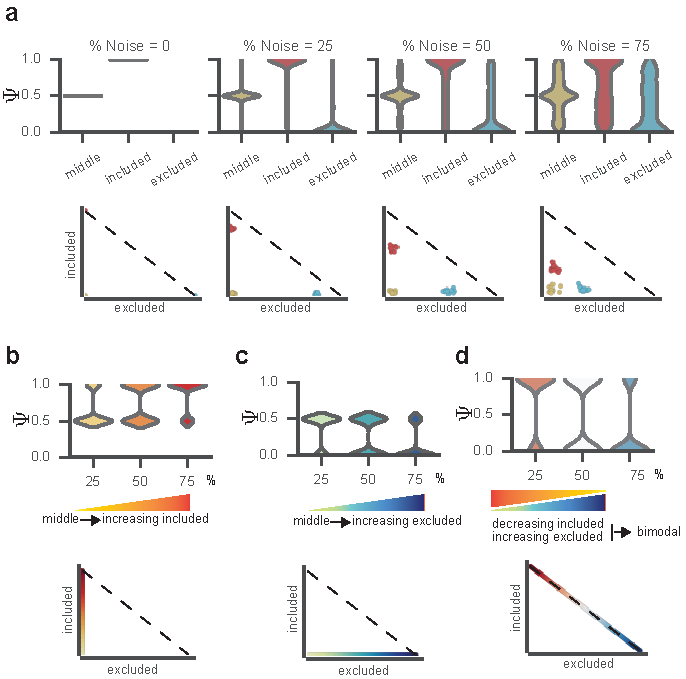
\includegraphics[width=5.8in]{figures/bonvoyage_simulations}
\end{figure}
%and, I'm not sure why, but one of the times I used this code the figure number wasn't augmented for the next figure, so check your figure numbers and if necessary uncomment the following line
\addtocounter{figure}{1}
\clearpage
% --- END manual facingcaption for bonvoyage simulations --- %

\subsection{Comparison to other methods}

As there exist many methods for comparing distributions, we will show that the magnitude of change obtained from \texttt{bonvoyage} is comparable to other metrics for assessing changes in distribution. In particular, we will show the metrics within each modality, and across modalities, compared to Jensen-Shannon Divergence \cite{Cover:2011vn} (JSD) in (\Cref{fig:bonvoyage_simulations}). While JSD is more sensitive to slight changes in distribution (their scatterplots are skewed towards the right), it does not also encode directionality of change. Thus, \texttt{bonvoyage} offers a unique perspective on how to interpret changes in distribution.

\section{Acknowledgements}

Chapter 2, in part, has been accepted for publication as the supplementary material as it may appear in Molecular Cell, 2017, Yan Song$^*$, Olga B Botvinnik$^*$, Michael T Lovci, Boyko Kakaradov, Patrick Liu, Jia L. Xu and Gene W Yeo ($^*$ These authors contributed equally to this work).  The dissertation author was one of the primary investigators and authors of this paper. 